\chapter{深度伪造的对抗性研究與近期研究發展}
\label{chap:4}

本作业在此章节分为三个部分,其一是针对于深度伪造的对抗性部分,这方面则可以从其深度伪造的生成面与检测面来看,其Li XR 等人近期来的汇整工作\cite{2021496} 有可以找到工作成果,另外还有 Yisroel Mirsky 等人 \cite{DBLP:journals/corr/abs-2004-11138} 对其 G工作与近来应用 Transformers 、增量学习在深度伪造领域的检测上的研究工作总结。


\section{深度伪造生成的对抗性}

由于近年来深度伪造技术所生成的人类脸部技术能够轻易修改人类的身分,甚至可以使目标人脸做出想要的脸部肌肉表情,使之在人脸身分辨识的领域遭遇到极大的挑战,同时因应人脸识别的对抗性攻击也不曾间断。其 Goswami G 等人 \cite{goswami2018unravelling},发现基于深度神经网络 (DNN) 架构的模型具有很高的表达能力和学习能力,然而,它们本质上是一种黑盒方法,因为在其多层表示中学习到的函数在数学上表示并不容易。意识到这一点后,许多研究人员已经开始设计方法来利用基于深度学习的演算法的缺点,质疑它们的鲁棒性并暴露它们的奇点。在在此研究中,研究者们试图解开与 DNN 在人脸识别方面的鲁棒性相关的三个方面:(i) 评估深度架构对人脸识别的影响,以应对攻击的脆弱性,这些攻击受到现实世界中普遍观察到的扭曲的启发,浅层学习方法和基于学习的对手可以很好地处理这些扭曲;(ii) 通过表征深层网络隐藏层中的异常滤波器响应行为来检测奇异点;和(iii) 对处理管道进行更正以缓解问题。该研究则使用多个开源的基于 DNN 的人脸识别网络(包括 OpenFace 和 VGG-Face)以及两个公开可用的资料库(MEDS 和 PaSC)的实验评估表明,基于深度学习的人脸识别算法的性能在存在这样的扭曲。同时该方法还与现有的检测算法进行了比较,结果表明,通过使用网络中隐藏层的响应适当地设计分类器,它能够以非常高的精度检测攻击。最后,研究提出了几种有效的对策来减轻对抗性攻击的影响并提高基于 DNN 的人脸识别的整体鲁棒性,其结果发现只要对图片与影像增加一定的遮挡或者在影像加入人类肉眼看不见得噪声,就能够有骗过机器的可能,该工作展示对 Parkhi OM 等人 \cite{parkhi2015deep} 所以提出 VGGface ,与 Baltrušaitis T 等人 \cite{baltruvsaitis2016openface} 所做的 Openface 等模型的实验。

\begin{figure}[htb]
\centering 
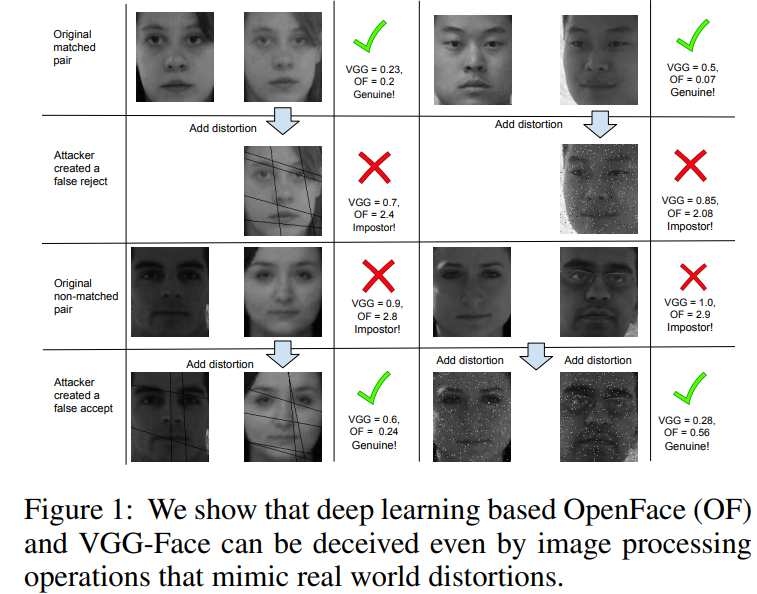
\includegraphics[width=0.90\textwidth]{img/ch4m0.png} 
\caption{ Goswami G 等人 \cite{goswami2018unravelling} }
\label{Test}
\end{figure}

Song Q 等人 \cite{yang2021attacks} 专注于一种对人脸识别网络进行攻击的新颖方法,该方法会误导网络将某人识别为目标人,而不是不明显地错误分类,同时,因为此缘故,研究者引入了一个特定的注意力对抗攻击生成网络来生成假人脸图像。为了捕获目标人的语义信息,这项工作添加了条件变分自动编码器和注意模块来学习人脸之间的实例级对应关系。与传统的双人 GAN 不同,这项工作引入了人脸识别网络作为第三个参与者参与生成器和判别器之间的竞争,这使得攻击者可以更好地模仿目标人。生成的结果难以引起旁观者注意的人脸可以逃避最先进网络的识别,并且大多数人都被识别为目标人。

\begin{figure}[htb]
\centering 
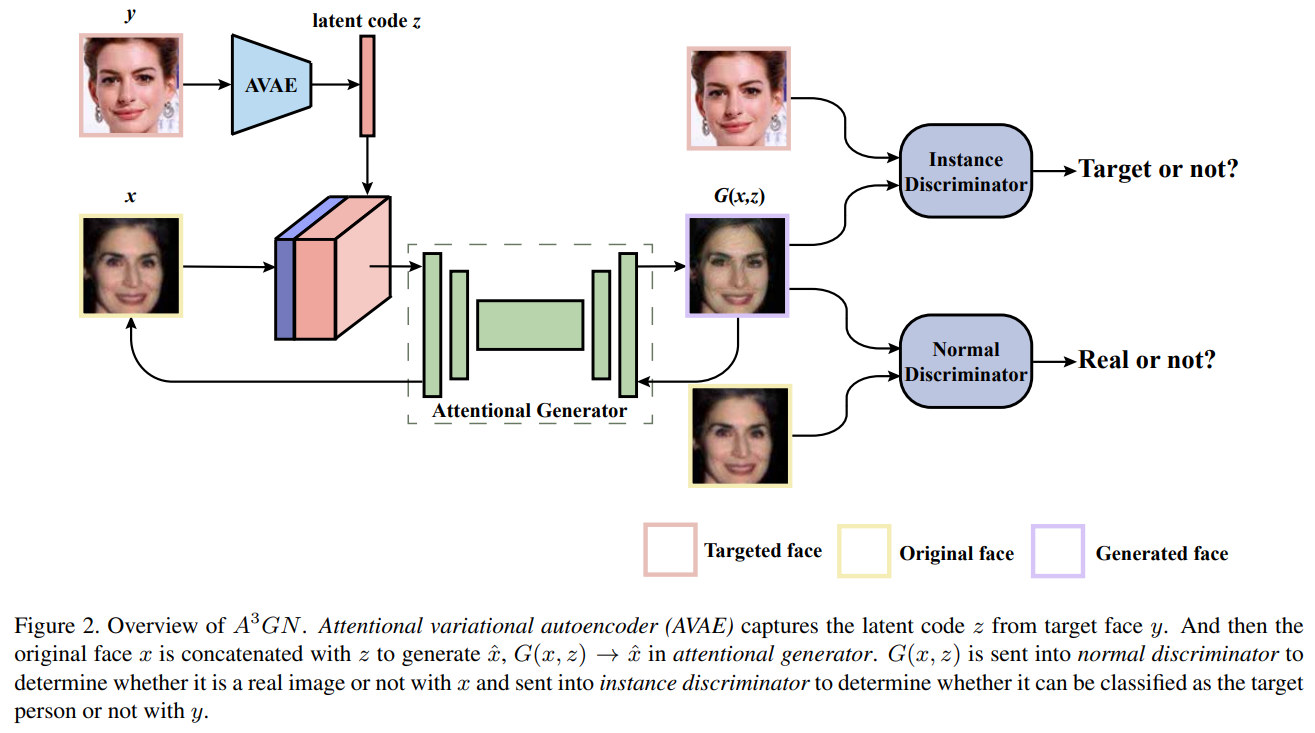
\includegraphics[width=0.90\textwidth]{img/ch4m1.png} 
\caption{ Song Q 等人 \cite{yang2021attacks} }
\label{Test}
\end{figure}

Majumdar P 等人 \cite{majumdar2019evading} 提出了部分面部篡改攻击,其中面部区域被替换或变形以生成篡改样本,而在 CMU-MultiPIE 数据集上使用两个最先进的人脸识别系统 VGG-Face 和 OpenFace 进行的人脸验证实验表明了这些系统对攻击的脆弱性。此外,该研究提出了一种部分人脸篡改检测(PFTD)网络来检测所提出的攻击,该网络通过结合输入图像的原始信息和高频信息来捕获原始图像和篡改图像之间的不一致性,以检测篡改图像。所提出的网络在篡改图像检测方面超越了现有基线深度神经网络的性能。

另外 Korshunov P 等人 \cite{korshunov2018deepfakes},通过使用预先训练的生成对抗网络 (GAN),将视频中的一个人的脸自动替换为另一个人的脸变得越来越容易。最近的公共丑闻,例如,名人的面孔被交换到色情视频上,需要自动检测这些 Deepfake 视频的方法,为了帮助开发此类方法,在本文中,我们展示了第一组从 VidTIMIT 数据库的视频中生成的公开可用的 Deepfake 视频。研究者使用基于 GAN 的开源软件来创建 Deepfakes,该研究强调训练和混合参数可以显著影响结果视频的质量。为了证明这种影响,研究者使用不同调整的参数集生成了具有低和高视觉质量的视频(每个 320 个视频),其研究展示了基于 VGG 和 Facenet 神经网络的最先进的人脸识别系统容易受到 Deepfake 视频的攻击,错误接受率分别为 85.62\% 和 95.00\%,这意味着检测 Deepfake 视频的方法是必要的。通过考虑几种基线方法,我们发现基于口型同步不一致检测的视听方法无法区分 Deepfake 视频。性能最佳的方法,基于视觉质量指标,常用于演示攻击检测领域,在高质量 Deepfakes 上的错误率为 8.97\%,最后的实验表明,GAN 生成的 Deepfake 视频对人脸识别系统和现有检测方法都具有挑战性,而人脸交换技术的进一步发展将使其变得更加困难。同样的也是 Korshunov P 等人 \cite{korshunov2019vulnerability} 展示了 Deepfake 视频的公开数据集,其中的人脸使用基于 GAN 的算法变形,同时为了生成这些影像,研究者使用了基于 GAN 的开源软件,并且我们强调训练和混合参数可以显著影响生成影像的品质,该研究表明,基于 VGG 和 Facenet 神经网络的最先进的人脸识别系统容易受到深度变形视频的影响,错误接受率分别为 85.62 和 95.00,这意味着检测这些视频的方法是必要的。同时研究也考虑了几种检测深度变形的基线方法,并发现基于视觉品质指标的方法(通常用于演示攻击检测领域)导致最佳性能,错误率为 8.97。而最后研究者的实验表明,GAN 生成的深度变形视频对人脸识别系统和现有检测方法都具有挑战性,而深度变形技术的进一步发展将使其更加如此。


\section{深度伪造检测的对抗性}

其深度伪造领域的演算法多数都是运用类神经网路等技术,而其神经网路模型本身即有着对抗样本的攻击,从 Szegedy C 等人 \cite{szegedy2013intriguing} 报告了两个这样的属性。首先,根据单元分析的各种方法,该研究发现单个高级单元和高级单元的随机线性组合之间没有区别。其研究表明,在神经网络的高层中,包含语义信息的是空间,而不是单个单元。其次,研究者们发现深度神经网络学习的输入-输出映射在很大程度上是不连续的。可以通过应用某种不可察觉的扰动来导致网络对图像进行错误分类,这种扰动是通过最大化网络的预测误差来发现的。此外,这些扰动的具体性质并不是学习的随机伪影:相同的扰动可能导致在数据集的不同子集上训练的不同网络对相同的输入进行错误分类。另 Goodfellow IJ 等人 \cite{goodfellow2014explaining} 认为神经网络易受对抗性扰动影响的主要原因是它们的线性性质,这种解释得到了新的定量结果的支持,同时给出了关于它们最有趣的事实的第一个解释:它们在架构和训练集上的泛化。此外,这种观点产生了一种简单而快速的生成对抗样本的方法。使用这种方法为对抗性训练提供示例,该研究减少了 MNIST 数据集上 maxout 网络的测试集误差。

\begin{figure}[htb]
\centering 
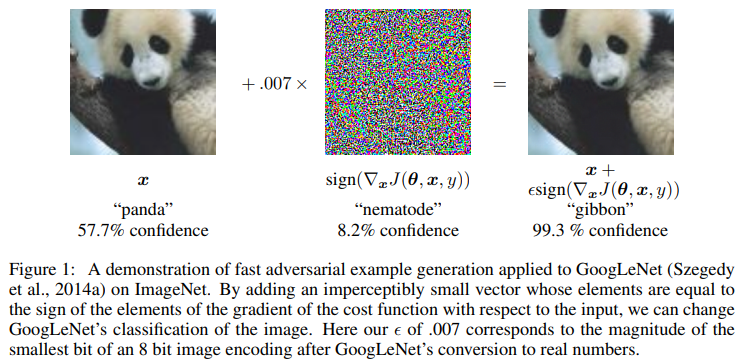
\includegraphics[width=0.90\textwidth]{img/ch4m2.png} 
\caption{ Goodfellow IJ 等人 \cite{goodfellow2014explaining} }
\label{Test}
\end{figure}

另外 Kurakin A 等人 \cite{kurakin2018adversarial} 发现大多数现有的机器学习分类器都非常容易受到对抗性示例的影响,对抗性示例是输入数据的样本,该样本经过了非常轻微的修改,旨在导致机器学习分类器对其进行错误分类。在许多情况下,这些修改可能非常微妙,以至于人类观察者甚至根本没有注意到修改,但分类器仍然会出错。对抗性示例会带来安全问题,因为它们可用于对机器学习系统进行攻击,即使对手无法访问底层模型。到目前为止,所有先前的工作都假设了一个威胁模型,其中攻击者可以将数据直接输入机器学习分类器。在物理世界中运行的系统并非总是如此,例如那些使用来自相机和其他传感器的信号作为输入的系统。该研究表明,即使在这样的物理世界场景中,机器学习系统也容易受到对抗性示例的影响。研究者们通过将从手机摄像头获得的对抗性图像馈送到 ImageNet Inception 分类器并测量系统的分类精度来证明这一点,最后研究者也发现,即使通过摄像头感知,大部分对抗性示例也被错误分类。

从上述几项研究的结果可以得知,这些由神经网络组成的模型在面对对抗性样本攻击时,会导致模型受到干扰,从而产生误判,由此也造成深度伪造技术在生成时可隐藏自身特征,从而绕过检测,由此有必要对当下的模型跟算法做对抗性的评估,另外 Wang SY 等人 \cite{kurakin2018adversarial} 研究尝试是否有可能创造一个“通用”检测器,用于将真实图像与 CNN 生成的图像区分开来,无论使用何种架构或数据集。为了测试这一点,研究者们收集了一个数据集,该数据集由 11 种不同的基于 CNN 的图像生成器模型生成的假图像组成,这些模型跨越当今常用架构的空间(ProGAN、StyleGAN、BigGAN、CycleGAN、StarGAN、GauGAN、DeepFakes、级联细化网络,隐式最大似然估计,二阶注意力超分辨率,在黑暗中看到)。其研究者证明,通过仔细的预处理和后处理以及数据增强,仅在一个特定的 CNN 生成器 (ProGAN) 上训练的标准图像分类器能够很好地泛化到看不见的架构、数据集和训练方法(包括刚刚发布的StyleGAN2)。而研究者的研究结果表明,当今 CNN 生成的图像存在一些常见的系统缺陷,从而阻止它们实现逼真的图像合成,这一有趣的可能性,同时该工作对训练资料进行类似于 JPEG 压缩、模糊等操作手法,可以提高模型的泛化性能。

另外 Neves JC 等人 \cite{neves2020ganprintr} 专注于整个面部图像的合成,这是一种特定类型的面部操作。该研究的主要贡献有四方面:i) 描述了一种从基于自动编码器的合成假图像中去除 GAN“指纹”的新策略,以欺骗面部操作检测系统,同时保持结果图像的视觉质量;ii) 对近期面部操作检测文献的深入分析;iii) 对这种类型的面部操作进行完整的实验评估,考虑到最先进的假检测系统(基于整体深度网络、隐写分析和局部伪影),并指出这项任务在不受约束的场景中的挑战性;最后 iv) 研究者们宣布了一个名为 iFakeFaceDB 的新型公共数据库,该数据库将该研究所提出的 GAN 指纹去除方法 (GANprintR) 应用于已经非常逼真的合成假图像。在该研究的实证评估中获得的结果表明,需要额外的努力来开发针对看不见的条件和欺骗技术的强大的面部操作检测系统,例如本研究中提出的技术。

Brockschmidt J 等人 \cite{brockschmidt2019generality} 
对都属于卷积神经网络 (CNN) 的 Rossler A 等人 \cite{rossler2019faceforensics++} 所做的的 Xception 与 Afchar D 等人 \cite{afchar2018mesonet} 所做的 Mesonet 进行对抗性评估,其实验使用来自六种最先进的面部伪造技术的样本:Deepfakes、Face2Face、FaceSwap、GANnotation、ICface 和 X2Face。研究者发现 MesoNet 和 XceptionNet 显示出泛化到多种欺骗技术的潜力,但在准确性上略有权衡,并且在很大程度上无法对抗看不见的技术。最后将这些结果松散地推断为类似的 CNN 架构,并强调需要更好的架构来应对普遍性的挑战。

Marra F 等人 \cite{marra2018detection} 研究了几种图像伪造检测器对图像到图像转换的性能,无论是在理想条件下,还是在存在压缩的情况下,通常在上传到社交网络时执行。该研究在 36302 张图像的数据集上进行,表明传统和深度学习检测器都可以实现高达 95\% 的检测精度,但只有后者在压缩数据上保持高达 89\% 的高精度,换言之现有的检测器若面对未知的压缩与类型,其表现并不理想。

Zhang X 等人 \cite{zhang2019detecting} 检测 GAN 生成的图像,传统的监督机器学习算法需要从目标 GAN 模型中收集大量真实和虚假图像。但是,攻击者使用的特定模型通常是不可用的。为了解决这个问题,该研究提出了一个 GAN 模拟器 AutoGAN,它可以模拟由几个流行的 GAN 模型共享的公共管道产生的伪影,此外,研究者确定了由通用 GAN 管道中包含的上采样组件引起的独特伪影。该研究从理论上表明,这种伪影表现为频域中光谱的复制,因此提出了一种基于光谱输入而不是像素输入的分类器模型。通过使用模拟图像来训练基于频谱的分类器,即使在训练期间没有看到目标 GAN 模型产生的假图像,此研究的方法在检测由流行 GAN 模型(如 CycleGAN)生成的假图像方面也取得了最先进的性能。

Du M 等人 \cite{du2019towards} 提出了 Locality-Aware AutoEncoder (LAE) 来弥补泛化差距。在训练过程中,研究者使用像素级掩码来规范 LAE 的局部解释,以强制模型从伪造区域学习内在表示,而不是在训练集中捕获伪影并学习表面相关性来执行检测。而该研究进一步提出了一个主动学习框架来选择具有挑战性的标签候选者,该框架需要不到 3\% 的训练数据使用人工蒙版,从而大大减少了规范化解释的注释工作。三个 deepfake 检测任务的实验结果表明,LAE 可以专注于伪造区域来做出决策。分析进一步表明,就先前未见过的操作的泛化精度而言,LAE 在三个深度伪造检测任务上的性能分别优于现有技术 6.52\%、12.03\% 和 3.08\%。

Huang, R 等人 \cite{huang2020security} 通过实验证明了个体对抗性扰动 (IAP) 和普遍对抗性扰动 (UAP) 的存在,它们可能导致表现良好的 FFM 行为不端。基于迭代过程,梯度信息用于生成两种可用于制造分类和分割输出的 IAP。相比之下,UAP 是在过火的基础上生成的。研究者们设计了一个新的目标函数,鼓励神经元过度激发,即使不使用训练数据也可以生成 UAP,实验证明了 UAP 在未见数据集和未见 FFM 之间的可转移性。此外,研究者对对抗性扰动的不可察觉性进行了主观评估,表明精心制作的 UAP 在视觉上可以忽略不计。这些发现为评估 FFM 的对抗性安全性提供了基准。

\section{深度伪造的生成与 GAN 分析}

从 Yisroel Mirsky 等人 \cite{DBLP:journals/corr/abs-2004-11138} 对其的工作中,认为生成式深度学习算法已经发展到难以区分真假的程度,而自 2018 年起,人们发现将这项技术用于不道德和恶意应用是多么容易,例如传播错误信息、冒充政治领导人以及诽谤无辜个人。从那时起,这些“深度伪造”取得了显著进展。该研究探讨了 deepfakes 的创建和检测,并深入了解这些架构的工作原理。

deepfake 这个词是“深度学习”和“假”两个词的组合,主要与人工神经网络(机器学习的一个分支)生成的内容有关。最常见的深度伪造形式涉及人类图像的生成和操纵。该技术具有创造性和生产性的应用。例如,外国电影的真实视频配音,通过历史人物的复活进行教育,以及在购物时虚拟试穿衣服。还有许多在线社区致力于为娱乐创建 deepfake 模因,例如描绘演员 Nicolas Cage 面孔的音乐视频。然而,尽管深度伪造的积极应用,该技术因其不道德和恶意方面而臭名昭著。

2017 年底,一位名为“deepfakes”的 Reddit 用户正在使用深度学习将名人的面孔转换为色情视频,并将其发布到网上。这一发现引起了媒体的狂热,此后大量新的 deepfake 视频开始出现。 2018 年,BuzzFeed 发布了一段前总统巴拉克·奥巴马 (Barak Obama) 就该主题发表演讲的 deepfake 视频。该视频是使用 Reddit 用户的软件 (FakeApp) 制作的,引发了对身份盗用、假冒和社交媒体上错误信息传播的担忧。

该研究将与人类视觉相关的深度伪造相应分类为四种,也就是重演(Reenactment)、替换(Replacement)、编辑(editing)和合成(synthesis)。尽管人类图像编辑和合成是活跃的研究课题,但重演和替换 deepfakes 是最受关注的问题,因为它们使攻击者能够控制自己的身份。尽管人类图像编辑和合成是活跃的研究课题,但重演和替换 deepfakes 是最受关注的问题,因为它们使攻击者能够控制自己的身份。在该篇论文中,研究者将 s 和 t 表示为源身份和目标身份,同时还将 $x_s$ 和 $x_t$ 表示为这些身份的图像,并将 $x_g$ 表示为从 s 和 t 生成的 deepfake。

\begin{figure}[htb]
\centering 
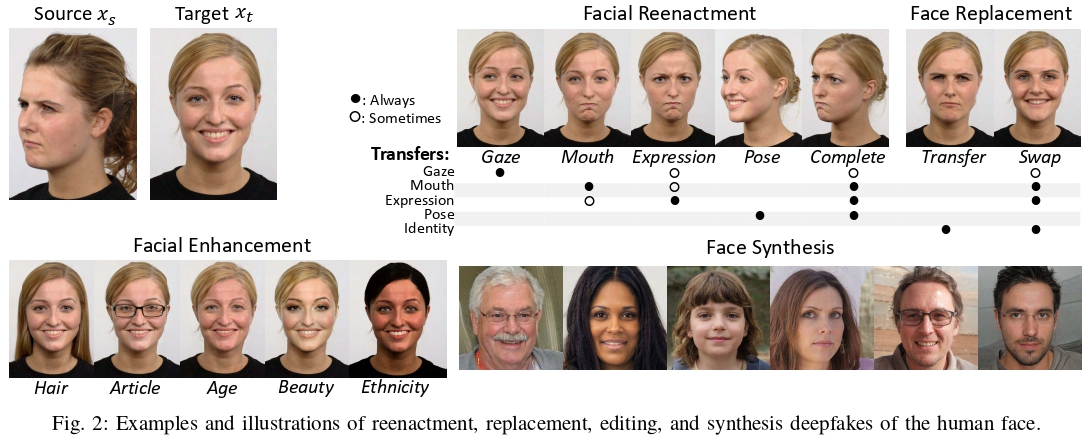
\includegraphics[width=0.90\textwidth]{img/ch4m3.png} 
\caption{ Yisroel Mirsky 等人 \cite{DBLP:journals/corr/abs-2004-11138} 深度伪造相应分类}
\label{Test}
\end{figure}


\subsection{重演 (Reenactment)}

重演 deepfake 是 $x_s$ 用于驱动 $x_t$ 的表情、嘴巴、凝视、姿势或身体的地方。其表达式重演是 $x_s$ 驱动 $x_t$ 表达式的地方
,这是最常见的重演形式,因为这些技术通常也会驱动目标的嘴巴和姿势,提供广泛的灵活性。在电影和视频游戏行业中发现了良性用途,在这些行业中演员的表演在后期进行了调整,并在教育媒体中重演了历史人物。

\begin{itemize}
\item [-] 嘴巴重演,也称为“配音”,是 $x_t$ 的嘴巴由 $x_s$ 的嘴巴驱动的地方,或者是包含语音的音频输入。该技术的良性用途包括将逼真的语音配音成另一种语言和编辑。
\item [-] 凝视重演是 $x_t$ 眼睛的方向和眼睑的位置由 $x_s$ 的驱动。这用于改善照片或在视频采访期间自动保持眼神交流。
\item [-] 姿势重演是 $x_t$ 的头部位置由 $x_s$ 驱动。该技术主要用于安全镜头中个人的面部正面化,并作为改进面部识别软件的一种手段。。
\item [-] 身体重演,也称为姿势转移和人体姿势合成,类似于上面列出的面部重演,只是它是驱动 $x_t$ 身体的姿势。
\item [-] 攻击模型。重演深度伪造使攻击者能够冒充身份,控制他或她所说或所做的事情。这使攻击者能够执行诽谤行为、造成不可信、传播错误信息和篡改证据。例如,攻击者可以冒充 t 来获得同事、朋友或家人的信任,以此作为获取金钱、网络基础设施或其他资产的手段。攻击者还可以出于勒索目的生成令人尴尬的 t 内容,或生成影响公众对个人或政治领袖的看法的内容。最后,该技术可用于篡改监控录像或其他一些档案图像,以试图在审判中植入虚假证据。
\end{itemize}

另外该研究将按时间顺序来回顾先前基于深度学习的重演部分,根据各个工作种类去提供了工作的总结和系统化。当中包含各个模型含出现时间与输出的结果,而且了解结果是影像还是图,同时还对应了嘴巴、凝视、身体等各项重演。

\begin{figure}[htb]
\centering 
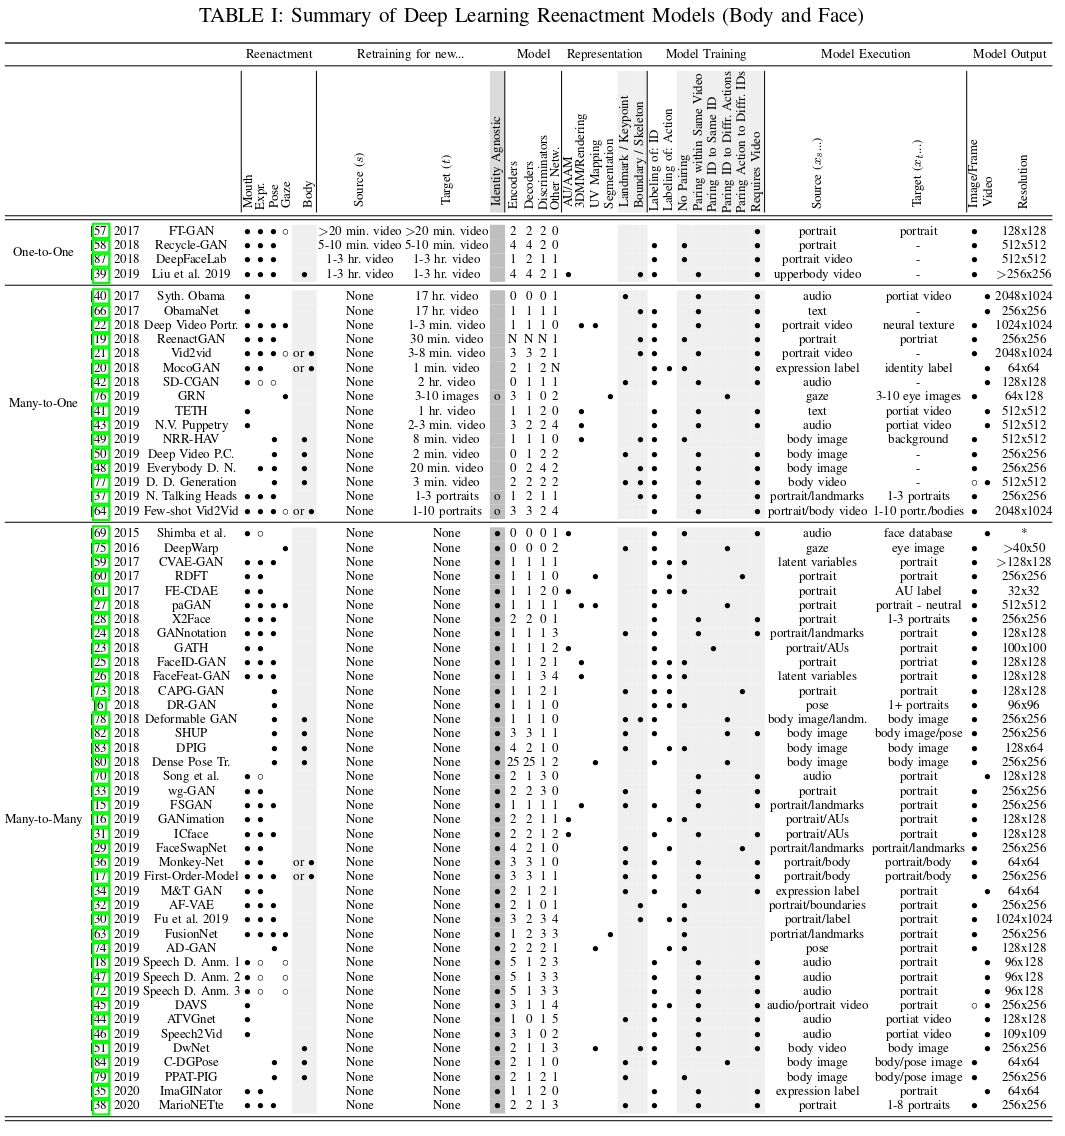
\includegraphics[width=1.10\textwidth]{img/ch4m5.png} 
\caption{ Yisroel Mirsky 等人 \cite{DBLP:journals/corr/abs-2004-11138} 深度伪造的重演 (Reenactment)工作总结}
\label{Test}
\end{figure}

另外针对表情重演又可以分为三类,其一为1)一对一 (One-to-One, Identity to Identity),Runze Xu 等人 CycleGAN 进行脸部重演,无需数据配对,s 和 t 的视频帧所在的两个域,为了避免 $x_g$ 中的伪影,研究者指出两个域必须如姿势和表情等共享相似的分布。另外在 2018 年时由 Bansal 等人提出了一个基于 CycleGAN 的通用翻译网络,称为 Recycle-GAN,其框架通过包含每个域的下一帧预测器网络来提高时间一致性并减轻伪影。对于脸部重演,研究者者训练他们的网络将 $x_s$ 的面部标志转换为 $x_t$ 的肖像。其二为多对一 (Many-to-One, Multiple Identities to a Single Identity),在2017 年时 Jianmin Bao 等人提出了 CVAE-GAN,这是一种条件 VAE-GAN,其中生成器以属性向量或类标签为条件,然而使用 CVAE-GAN 重新制定需要在类似于在目标姿势之间通过插值潜在变量进行手动属性变形,后来在 2018 年时,发布了大量与源身份无关的模型,其每个模型都提出了一种不同的方法来将 s 与 t 进行解耦,而所谓的面部边界转换,是一种方法是首先将源面部边界的结构转换为目标的面部边界结构,然后再将它们传递给生成器。如框架 "ReenactGAN" 的研究者使用 CycleGAN 将边界 $b_s$ 转换为目标的面部形状作为 $b_t$ ,然后使用类似 pix2pix 的生成器生成 $x_g$。最后则是多对多 (Many-to-Many, Multiple IDs to Multiple IDs),当中身份不可知模型的首次尝试是在 2017 年,Kyle Olszewski 等人使用 conditional GAN(CGAN)来完成任务,其方法是 (1) 将内面区域提取为 ($x_t$, $x_s$),然后 (2) 将它们传递给 ED 以产生 $x_g$ 受到 $L_1$ 和 $L_{adv}$ 损失,同时使用 CGAN 的挑战在于必须对训练数据进行配对,比如具有相同表情的不同身份的图像。更进一步来说,在 Yuqian Zhou 等人的工作中,作者以低分辨率重新制作了完整的肖像,他们的方法是将身份解耦,即使用条件对抗自动编码器将身份与潜在空间中的表达式分离。然而,他们的方法仅限于使用捕获 $x_s$ 的谨慎 AU 表达式标签(固定表达式)来驱动 $x_t$。最后则是 Yisroel Mirsky 等人 \cite{DBLP:journals/corr/abs-2004-11138} 在其工作针对人类脸部的重演进行整理如他们的表所示。

\begin{figure}[htb]
\centering 
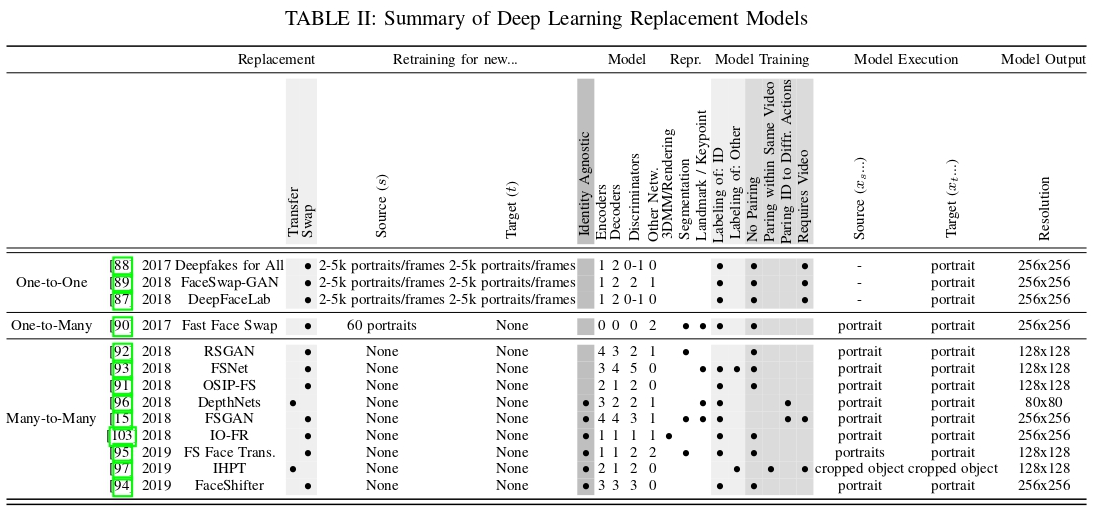
\includegraphics[width=1.10\textwidth]{img/ch4m10.png} 
\caption{ Yisroel Mirsky 等人 \cite{DBLP:journals/corr/abs-2004-11138} 在其工作针对人类脸部的重演}
\label{Test}
\end{figure}

\subsection{更换 (Replacement)}

替换 deepfake 是将 $x_t$ 的内容替换为 $x_s$ 的内容,保留 s 的身份。转移是将 $x_t$ 的内容替换为 $x_s$ 的内容。一种常见的转移类型是面部转移,在时尚行业中用于形象化穿着不同服装的个人。交换是从 $x_s$ 传输到 $x_t$ 的内容由 $x_t$ 驱动的地方。最流行的交换替换类型是“面部交换”,通常用于通过将演员的身份与名人的身份交换来生成模因或讽刺内容。换脸的另一个良性用途包括在公共内容中匿名化一个人的身份,而不是模糊或像素化。

当中要注意的是攻击模型,其替换 deepfakes 以其有害应用而闻名。例如复仇色情是攻击者将受害者的脸换到色情女演员的身上,以羞辱、诽谤和勒索受害者。换脸也可以用作通过将 t 的脸转移到相似的身体上来完全重现 t 的捷径。这种方法过去曾被用作传播政治观点的工具。


\subsection{增强 (Enhancement)}

一个结界 deepfake 是 $x_t$ 的属性所在被添加、更改或删除。一些例子包括改变目标的衣服、面部毛发、年龄、体重、美丽和种族。 FaceApp 等应用程序使用户能够改变他们的外观以进行娱乐和轻松编辑多媒体。攻击者可以使用相同的过程来建立虚假角色以误导他人。例如可以让生病的领导者看起来很健康,而儿童或性侵犯者可以改变他们的年龄和性别来建立在线动态档案。增强深度伪造的一个已知不道德使用是为了羞辱或娱乐而脱掉受害者的衣服。

\subsection{合成 (Synthesis)}

合成是在没有目标作为基础的情况下创建 deepfake $x_g$ 的地方。人脸和身体合成技术,例如可以创建免版税影视素材或为电影和游戏生成角色。但是,与增强 deepfakes 类似,它也可用于在线创建虚假角色。

\subsection{深度伪造的组合与变体}

\begin{figure}[htb]
\centering 
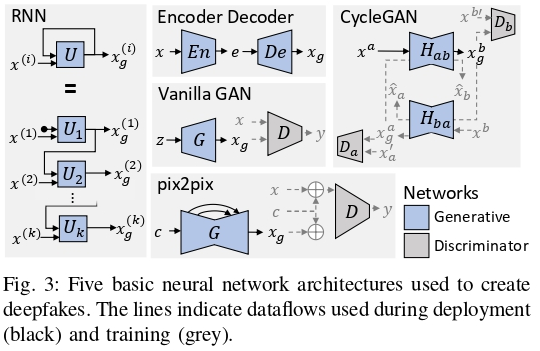
\includegraphics[width=0.90\textwidth]{img/ch4m4.png} 
\caption{ Yisroel Mirsky 等人 \cite{DBLP:journals/corr/abs-2004-11138} 深度伪造组合或变体}
\label{Test}
\end{figure}

深度伪造通常是使用六个不同网络的组合或变体创建,第一种为编码器-解码器网络 (ED)。一个 ED 至少由两个网络组成,一个编码器 En 和一个解码器 De。 ED 的中心层较窄,因此当它被训练为 De(En(x)) = xg 时,网络被迫总结观察到的概念。给定分布 X,x 的摘要是 En(x) = e,通常被称为编码或嵌入,而 E = En(X) 被称为“潜在空间”。

当然 Deepfake 技术通常使用多个编码器或解码器并操纵编码以影响输出 $x_g$。如果编码器和解码器是对称的,并且使用目标 De(En(x)) = x 训练网络,则该网络称为自编码器,输出是 x 的重建,表示为 $\hat{\boldsymbol{x}}$。另一种特殊的 ED 是变分自动编码器 (VAE),其中编码器学习给定 X 的解码器的后验分布。 VAE 比自动编码器更擅长生成内容,因为潜在空间中的概念被解开,因此编码对插值和修改的响应更好。

第二种为卷积神经网络 (CNN),全连接(密集)网络相比,CNN 学习数据中的模式层次结构,因此在处理图像方面效率更高。 CNN 中的卷积层学习过滤器,这些过滤器在输入上移动,形成抽象特征图作为输出。当网络变得更深时,池化层用于降低维数,而上采样层用于增加它。通过卷积、池化和上采样层,可以为图像构建 ED CNN。

在此要注意的为生成对抗网络 (GAN),其GAN 于 2014 年由 Goodfellow 等人首次提出。 GAN 由两个相互对抗的神经网络组成了生成器 G 和判别器 D。 G 创建假样本 xg 的目的是欺骗 D,并且 D 学会区分真实样本 (x ∈ X) 和假样本 ($x_g$ = G(z),其中 z ∼ N)。具体来说,有一个对抗性损失用于分别训练 D 和 G。这种零和游戏导致 G 学习如何生成与原始分布无法区分的样本,训练后丢弃 D,使用 G 生成内容,当应用于图像时,这种方法会产生照片般逼真的图像,其数学式如下 :

$$
\begin{gathered}
\mathcal{L}_{a d v}(D)=\max \log D(x)+\log (1-D(G(z))) \\
\mathcal{L}_{a d v}(G)=\min \log (1 D(G(z)))
\end{gathered}
$$

第三种为 Image-to-Image Translation (pix2pix),过去人们提出了对 GAN 的许多变化和改进。一个流行的版本是 pix2pix 框架,它可以实现从一个图像域到另一个域的转换。在 pix2pix 中,G 尝试在给定视觉上下文 xc 作为输入的情况下生成图像 xg,并且 D 区分 (x, $x_c$) 和 ($x_g$, $x_c$)。此外,G 是一个 ED CNN,具有从 En 到 De 的跳跃连接(称为 U-Net),它使 G 能够在需要时绕过压缩层来生成高保真图像。后来,pix2pixHD 被提出用于生成具有更好保真度的高分辨率图像。第四种为 CycleGAN 为 pix2pix 的改进,可通过非配对训练实现图像翻译。该网络形成一个由两个 GAN 组成的循环,用于将图像从一个域转换到另一个域,然后再返回以确保与循环一致性损失 (Lcyc) 的一致性,最后第五种 Recurrent Neural Networks (RNN) 是一种可以处理顺序和可变长度数据的神经网络。网络在处理 x(i - 1) 后会记住内部状态,并可以使用它来处理 x(i) 等等。在 deepfake 创建中,RNN 通常用于处理音频,有时也用于处理视频,更外高级的 RNN 版本包括长短期记忆 (LSTM) 和门循环单元 (GRU)。



\section{Transformers 與 增量学习}



